\section{Introduzione}
  \begin{frame}{Math packages}

    \begin{itemize}
      \item<1-> Pacchetto \texttt{\textcolor{blue}{amsmath}}
      \item<2-> Pacchetto \texttt{\textcolor{blue}{amssymb}}
	  \item<3-> \texttt{\textcolor{blue}{\textbackslash usepackage\{amsmath, amssymb\}}}
    \end{itemize}

    \begin{itemize}
      \item<4-> Formule ``in linea'' $a^2 + b^2 = c^2$
      \item<5-> Formule ``in display''
      \begin{itemize}
        \item[]<5-> \begin{equation} e^{i\pi}+1=0 \end{equation}
      \end{itemize}
    \end{itemize}
    
    \begin{textblock*}{5cm}(9cm,2.5cm)
      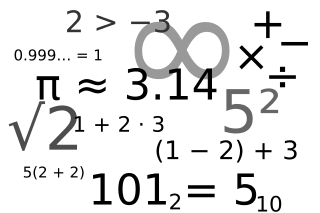
\includegraphics[scale=0.25]{math_symbols}
    \end{textblock*}

\end{frame}
